\section{Compactness}
$E\subset X$ is compact if from any open covering $\{ A_i\}_{i\in I}$ ($A_i$ open $\forall i\in I$, $E\subset \bigcup_{i\in I}A_i$) we can extract a finite subcovering.\\
Typically, we can take $E$, fix $r>0$, consider $\{ B_r(x)\}_{x\in E}$. Then $$E\subset \bigcup_{x\in E}B_r(x)$$
If $E$ is compact, $\exists x_1,x_2,\dots, x_k\in E$ s.t. $$E\subset \bigcup_{i=1}^k B_r(x_i)$$
\subsubsection{(def) Sequentially compact}
$E$ is sequentially compact if $\forall \{x_n\}_{n\in \mathbb N}\subset E$,
$$\exists \{ x_{n_k}\} \text{ convergent in }E$$
\subsubsection{(def) Relatively compact set}
$E\subset X$ is relatively compact if $\overline E$ is compact
\subsection{Finite dimension}
\subsubsection{(thm) Heine-Borel}
Consider $(X,\cnorm )$ a normed vector space. If $\dim (X)<+\infty$,
$$E \text{ compact }\iff E \text{ closed and bounded}$$
\paragraph{Remark}
If $\dim(X)=+\infty$,
$$E\text{ compact}\substack{\implies\\ \centernot\impliedby} E\text{ closed and bounded}$$
\subsection{Infinite dimension}
\subsubsection{(thm) Riesz}
Take any normed vector space $(X,\cnorm)$, \\
take the ball of radius 1 and centered in origin $$\overline{B_1(0)}\text{ is compact }\iff \dim(X)<+\infty$$
\begin{proof}\ \\
$\impliedby$: see analysis 1,2 + equivalent norms\\
$\implies$: assume that $\overline{B_1(0)}=\{ x\in X: \Vert x\Vert \leq 1\}$ is compact.\\
Consider $\{B_{\frac 12}(x)\}_{x\in \overline{B_1(0)}}$\\
($B_{\frac 12}(x)=\{y\in X:\Vert x-y\Vert <\frac 12\}$)\\
Then $$\overline{B_1(0)}\subset \bigcup_{x\in \overline{B_1(0)}}B_{\frac 12}(x)$$
By compactness, $\exists\ x_1,x_2,\dots,x_k\in \overline{B_1(0)}$ s.t.
$$\overline{B_1(0)}\subset \bigcup_{i=1}^kB_{\frac 12}(x_i)\subset \bigcup_{i=1}^k\overline{B_{\frac 12}(x_i)}$$
This means that:
    $$\forall x\in \overline{B_1(0)}\quad \exists\ i\in \{1,\dots,k\},\quad \exists \ z:\Vert z\Vert \leq \frac 12\quad \text{ s.t. }x=x_i+z$$
Define $V=span\{x_1,\dots,x_n\}$ \\
Then $V\subset X$ is a vector subspace and $dim(V)\leq k<+\infty$\\
Then we can rewrite:
$$\forall x\in \overline{B_1(0)}\quad \exists\ v\in V,\quad \exists \ z\in X:\Vert z\Vert \leq \frac 12\quad \text{ s.t. }x=v+z$$
Take $y\in X(y\neq0)\implies \frac{y}{\Vert y\Vert}\in \overline{B_1(0)}$ and $\exists v\in V, \ z:\Vert z\Vert \leq \frac 12$ s.t. 
$$\frac y{\Vert y\Vert}=v+z$$
i.e.
$$y=v\Vert y\Vert+z\Vert y\Vert $$
Defining $v'\coloneqq v\Vert y\Vert$, $z'\coloneqq z\Vert y\Vert$,
$$y=v'+z'$$
where $v'\in V, \ \Vert z'\Vert \leq \frac{\Vert y\Vert}{2}$\\
Take any $x\in X$, apply the last result to $y=x$.
$$x=v_1+z_1$$
where $v_1\in V, \ \Vert z_1\Vert \leq \frac{\Vert x\Vert}2$.\\
apply again, to $y=z_1$\\
$$x=v_1+v'+z'$$
$v'\in V$, $\Vert z'\Vert \leq \frac{z_1}2\leq \frac{\Vert x\Vert}4$\\
$v_2 = v_1+v'$, $z'=z_2$\\
$$x =v_2+z_2$$
$$v_2\in V, \ \Vert z_2\Vert \leq \frac 14 \Vert x\Vert$$
By induction, ...
$$x=v_n+z_n$$
where $v_n\in V, \ \Vert z_n\Vert \leq \frac 1{2^n}\Vert x\Vert$\\
Then:
$$z_n\xrightarrow[n\to+\infty]{}0$$
$$v_n=x-z_n\xrightarrow[n\to+\infty]{}x$$
$$\begin{cases}
    \{v_n\}\subset V\\v_n\to x\in X
\end{cases}\implies x\in V$$
$$dim(V)<+\infty\implies V\text{ is closed}$$
I have shown that $$\forall x\in X\implies x\in V$$
i.e. $X=V$ and $dim (X)\leq k<+\infty$
\end{proof}
\subsection{Compactness in $C([a,b])$}
We always consider $(C([a,b]),\cnorm_\infty)$ which is a Banach space.
$$\Vert u\Vert_\infty =\max_{x\in [a,b]}|u(x)|$$
(one may deal with $C(Q)$ with $Q\subset \mathbb R^n$ closed and bounded).
\subsubsection{(def) Uniform Equicontinuity of a sequence}
Take $\{u_n\}_{n\in \mathbb N}\subset C([a,b])$ is uniformly equicontinuous if $$\forall \varepsilon>0,\ \exists\ \delta >0 \text{ s.t. }|x-y|<\delta$$ 
$$\implies |u_n(x)-u_n(y)|<\varepsilon\quad \forall x,y\in [a,b], \ \forall n\in \mathbb N$$
This means that every functions $u_n$ in the sequence behaves similarly in terms of continuitym with the same $\delta$ working for all functions in the sequence, not just for a specific function.

\paragraph{remarks}
\begin{itemize}
    \item In the pointwise continuity definition of $u$ in $x_0$, we have:
    $$ \delta = \delta(u,x_0,\varepsilon)$$
    \item In the uniform continuity definition of $u$, we have:
    $$ \delta = \delta(u,\varepsilon)$$
    \item In the uniform equicontinuity of $\{u\}_n$ we have:
    $$\delta = \delta(\varepsilon)$$
\end{itemize}
This progression from pointwise continuity to uniform continuity reflects increasing uniformity in the way continuity is controlled across different functions and points.
\subsubsection{(thm) Ascoli-Arzelà}
Take $\{u_n\}_{n\in \mathbb N}\subset C([a,b])$.\\
Assume:
\begin{itemize}
    \item $\{u_n\}_{n\in \mathbb N}$ is unif. bounded
    $$\Vert u_n\Vert_\infty\leq M\quad\forall n$$
    \item $\{u_n\}_{n\in \mathbb N}$ unif. equicontinuous
\end{itemize}
Then:\\
$\exists$ a subsequence $\{u_{n_k}\}_{k\in \mathbb N}$ and $u\in C([a,b])$ s.t. $u_{n_k}\xrightarrow[k\to+\infty]{}u$
\paragraph{Example} $\{u_n\}\subset C^1([a,b])\subset C([a,b])$.\\
Assume that
\begin{enumerate}
    \item $\Vert u_n\Vert_\infty \leq M\quad \forall n$
    \item $\Vert u'_n\Vert_\infty\leq L\quad \forall n$
\end{enumerate}
(for some constants $M,L\geq 0$)\\
Then the theorem applies. Indeed:
\begin{enumerate}
    \item $\implies$ i) in Ascoli-Arzelà thm.
\end{enumerate}
To check equicontinuity: $\forall x,y\in[a,b], \quad x\neq y$
$$|u_n(x)-u_n(y)|=|u'_n(\xi)\cdot (x-y)|$$
(by Lagrange mean value theorem, $\xi$ in the smaller interval)
$$|u_n(x)-u_n(y)|\leq|u'_n(\xi)|\cdot|x-y|\leq \Vert u'_n\Vert_\infty\cdot|x-y|\leq L|x-y|\quad ,\forall n$$
$\implies$ Equicontinuity: $\forall \varepsilon $ take $\delta =\frac \varepsilon L$
Roughly:
$$\text{"boundedness in }C^1\implies \text{ compactness in }C^0\text{"} $$
\paragraph{rmk}
The same is true for Lipschitz continuous functions with uniformly bounded Lipschitz constant
\paragraph{rmk}
there are similar theorems in $L^p, \dots W^{1,p}$
$$\text{"boundedness in }W^{1,p}\implies \text{ compactness in }L^p\text{"} $$
\subsection{Density, Separability}
$(X,d)$ metric space.
\subsubsection{(def) dense space}
$D\subset X$ is dense if $\overline{D}=X$ ($\forall x\in X\quad \exists \{y_n\}_n\subset D : \ y_n\to x\text{ in }X$)
\subsubsection{(def) separable space}
$X$ is separable if $\exists D\subset X$, $D$ countable and dense.
\paragraph{rmk} tipically, one uses dense subsets because "continuous properties, true on $D$, are true in $X$".\\
When $D$ is separable, you have few elements to check the property.
\paragraph{Example}
$\mathbb R,\ \mathbb R^n,\ \Omega \subset \mathbb R^n$ are all separable: $\overline{\mathbb Q}=\mathbb R$ and $\mathbb Q$ is countable.
\subsubsection{(thm) Separability of functional spaces ($C,\ L^p, L^\infty$)} %thm??? maybe a remark...
\begin{itemize}
    \item $(C([a,b]), \cnorm_\infty)$ is separable
    \item $(L^p(\mathbb R), \cnorm_p)$ is separable if $1\leq p<+\infty$
    \item $(L^\infty(\mathbb R),\cnorm_\infty)$ is not separable
\end{itemize}
\subsubsection{(thm) Stone-Weierstrass}
"Polynomials" are dense in $C([a,b])$
(and polynomials with coefficients in $\mathbb Q$ are countable and dense)
\paragraph{Alternative statement (Wikipedia)}
Also known as "Weierstrass approximation theorem", states that every continuous function defined on a closed interval $[a,b]$ can be uniformly approximated as closely as desired by a polynomial function.
\paragraph{Explaination}
The functions belonging to $C([a,b])$ take real values in the interval $[a,b]$ and are equipped with the sup norm ($\cnorm_\infty$ norm): $$\Vert f-g\Vert =\sup_{x\in [a,b]}|f(x)-g(x)|$$
this norm measures the maximum difference between two functions over the interval $[a,b]$. 

Saying that polynomials are dense in $C([a,b])$ means that for any continuous function $f\in C([a,b])$ and any given $\varepsilon>0$, there exists a polynomial $p(x)$ s.t. $$\Vert f-p\Vert <\varepsilon$$.
\subsection{Dense subspaces of $L^p(\mathbb R)$}
\paragraph{Recall}
$s$ is (measurable and) simple function \\$s:\mathbb R\to\mathbb R$ s.t.
$$s=\sum_{i=1}^ka_i\rchi_{E_i}$$
where
\begin{itemize}
    \item $a_i\in \mathbb R$ (distinct)
    \item $E_i\in \mathcal L(\mathbb R)$ (disjoint)
    \item $\bigcup E_i=\mathbb R$
\end{itemize}
We know that $s$ simple $\implies$ $s \in L^\infty(\mathbb R)$
\paragraph{Question}
Does $s\in L^p(\mathbb R)$ (with $1\leq p<+\infty$)?
\paragraph{Answer}
$$s\in L^p(\mathbb R)\iff \lambda\Big (\{x:s(x)\neq0\}\Big)<+\infty$$
$\tilde{\mathcal S}(\mathbb  R)\coloneqq\lambda\Big (\{x:s(x)\neq0\}\Big)$
\subsubsection{(thm) $\tilde S(\mathbb R)$ is dense in $L^p(\mathbb R)$}
$\tilde{\mathcal S}(\mathbb R)$ is dense in $L^p(\mathbb R)\quad \forall \ 1\leq p<+\infty$

\subsubsection{(def) support}
\begin{itemize}
    \item $u:\mathbb R\to \mathbb R$. The support of $u$ is $$supp(u)=\overline{\{x\in \mathbb R : \ u(x)\neq 0}$$
    \item $C_c(\mathbb R)=\{ u\in C(\mathbb R): \ supp(u)$ is compact$\}$
    \item $C_c^\infty(\mathbb R)=C_0^\infty(\mathbb R)=\mathcal D(\mathbb R)$
\end{itemize}
\subsubsection{(thm) $C_c^\infty$ density in $L^p(\mathbb R)$}
$C_c^\infty(\mathbb R)$ is dense in $L^p(\mathbb R)$ $\forall\ 1\leq p<+\infty$\\
By consequence, also $C_c(\mathbb R)$ is dense, etc.
\subsubsection{(rmk) $C_c(\mathbb R)$ is not dense in $L^\infty(\mathbb R)$}
$C_c(\mathbb R)\subset L^\infty(\mathbb R)$ is not dense (i.e. the space of continuous function with compact support in $\mathbb R$ is not dense in the space of essentially bounded functions).

Saying that $C_c(\mathbb R)$ is dense in $L^\infty(\mathbb R)$ would mean that any function in $L^\infty(\mathbb R)$ could be approximated arbitrarily closely (in the $\cnorm_\infty$ norm) by functions from $C_c(\mathbb R)$.


Take
$$\mathcal H(x) =\begin{cases}
    1\quad x\geq0\\0\quad x<0
\end{cases}$$
We observe that $\mathcal H(x)$ is clearly a function $\in L^\infty(\mathbb R)$ since it can be bounded with $\Vert\mathcal H\Vert_\infty=1$.\\
Suppose now to pick a function $g\in C_c(\mathbb R)$ s.t. $\Vert \mathcal H-g\Vert_\infty \leq \frac 13$ (i.e. $| \mathcal H-g| \leq \frac 13$ a.e. $x\in \mathbb R$)

$$\mathcal H(x)-\frac{1}{3}\leq g\leq \mathcal H(x)+\frac 13\quad , \forall x\in \mathbb R$$
\begin{figure}[h]
    \centering
    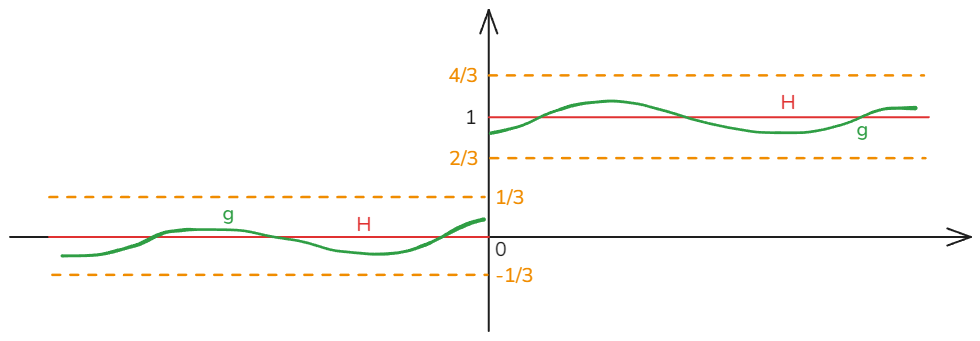
\includegraphics[width=0.9\linewidth]{assets/heaviside_cartoon.png}
    \caption{Graph of $\mathcal H(x)$ and $g(x)$}
    \label{fig:enter-label}
\end{figure}

We immidiately notice that $g$ can't be a continuous function in $x=0$, since the left-hand and the right-hand limits doesn't agree.\\
$\implies \ g$ $\mathcal H(x)$ can't be approximated arbitrarily closely in $\cnorm_\infty$-norm by any $g\in C_c(\mathbb R)$. Thus, $C_c(\mathbb R)$ is not dense in $L^\infty(\mathbb R)$.

\subsubsection{(lemma) Non-separable Banach spaces}
Take any $X$ Banach space (assumption may be restricted, we use Banach for simplicity)\\
Assume that $\{A_i\}_{i\in I}$ is s.t.
\begin{itemize}
    \item $\forall i\in I,\ A_i\subset X$ open, non empty
    \item $A_i\cap A_j=\emptyset\quad \forall i\neq j$
    \item $I$ is more than countable
\end{itemize}
Then $X$ is not separable
\begin{proof}
    By contradiction, assume $X$ separable, and so there is a countable dense subset $\{x_n\}$ of $X$:
    $$\exists\ \{x_n\}_{n\in \mathbb N}\subset X\text{ s.t. } X=\overline{\bigcup_{n\in \mathbb N}\{x_n\}}$$
    
    $\forall A_i \ ,\exists\ x_{n(i)}\in A_i$
    \begin{enumerate}
        \item $A_i$ not empty $\implies \exists\ z_i\in A_i$
        \item $\{x_n\}$ dense $\implies x_{n_k}\to z_i$
        \item $A_i$ open $\implies$ the sequence enters $A_i$
    \end{enumerate}
    Since $A_i\cap A_j=\emptyset \quad \forall i\neq j$
    then $x_{n(i)}\neq x_{n(j)}$ i.e. $n(i)\neq n(j)$\\
    We have a map
    $$I\in i \xrightarrow[\quad\quad]{}n(i)\in \mathbb N$$ is injective
    $\implies I$ is at most countable, contradiction
\end{proof}
\subsubsection{(thm) $L^\infty(\mathbb R)$ is not separable}
\begin{proof}
    We use the above lemma.\\
    $\forall \alpha\in \mathbb R^+=(0,+\infty)$\\
    $\alpha_1\quad -\alpha_1\quad \alpha_2\quad -\alpha_2$
    take $$g_\alpha (x)=\rchi_{[-\alpha, \alpha]}(x)=\begin{cases}
        1\quad |x|\leq \alpha \\
        0\quad |x|>\alpha
    \end{cases}$$
$$\alpha_1\neq \alpha_2 \implies \Vert g_{\alpha_1}-g_{\alpha_2}\Vert_\infty=1$$

\begin{figure}[H]
    \centering
    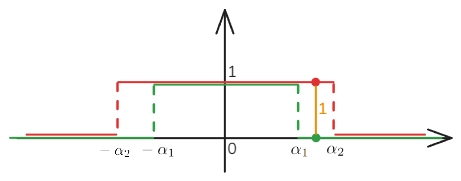
\includegraphics[width=0.5\linewidth]{assets/g_alpha1&2.png}
    \caption{$\Vert g_{\alpha_1}-g_{\alpha_2}\Vert_{\infty}=1$ (orange segment)}
    \label{fig:enter-label}
\end{figure}
$\implies B_{1/2}(g_{\alpha_1})\cap B_{1/2}(g_{\alpha_2})=\emptyset $
\begin{figure}[H]
    \centering
    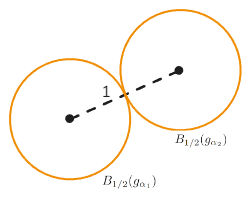
\includegraphics[width=0.3\linewidth]{assets/12balls_in_g_alpha.png}
    \label{fig:enter-label}
\end{figure}
$\forall f\in L^\infty(\mathbb R)$,\\
$$1=\Vert g_{\alpha_1}-g_{\alpha_2}\Vert_\infty\leq \Vert g_{\alpha_1}-f\Vert_\infty +\Vert f-g_{\alpha_2}\Vert_\infty$$ one of them is $>\frac 12$
Then we can apply the lemma using $\{B_{\frac12}(g_\alpha)\}_{\alpha\in (0,+\infty)}$ since it is:
\begin{itemize}
    \item Open
    \item Non-empty
    \item Disjoint
    \item $(0,+\infty)$ is more than countable
\end{itemize}
\end{proof}
